\chapterhead{4}{Trading Keys}{Seeing whether someone else gets the same answer}\label{ch4}

A key can seem perfect to the person who made it, because the maker knows what every question means. A test of a key is whether \emph{someone else} using it gets the same answer.

\begin{tryit}{Trade keys with a friend}
\textbf{You need:} ten buttons or small things, a key you wrote, and a friend.
\begin{enumerate}[leftmargin=1.6em]
\item Write a key with three yes-or-no questions for your ten things. Sort the ten things yourself and note where each ends.
\item Give your friend the key and the ten things, without telling them where each goes.
\item Ask your friend to sort them using only the key.
\item Count how many things ended in the same place for both of you.
\end{enumerate}
\par\medskip
\renewcommand{\arraystretch}{1.6}
\begin{tabular}{|l|c|c|c|}
\hline
 & \textbf{Things sorted} & \textbf{Same group both times} & \textbf{Different group}\\ \hline
\textbf{Count} & 10 & & \\ \hline
\end{tabular}
\end{tryit}

\begin{worked}{Practice numbers, not from a real test}
Ten buttons. My friend agreed with me on 8 and disagreed on 2. Agreement: 8 of 10.\\
The two disagreements were both on the question ``Is it big?'' My friend and I drew the line in different places.\\
I rewrote the question as ``Is it wider than 2~cm?'' and tried again. This time my friend agreed on all 10.
\end{worked}

\begin{center}
\begin{tikzpicture}
  \node[bigcir,minimum size=2.4cm] (a) at (0,0) {}; \node[font=\sffamily\scriptsize,align=center] at (0,0) {``Is it big?''\\8 of 10};
  \node[wrapcir,minimum size=2.9cm] (w) at (5.2,0) {}; \node[font=\sffamily\scriptsize,align=center] at (5.2,0) {``Wider than\\2 cm?''\\10 of 10};
  \draw[popA] (a) -- node[above,note] {rewrite} (w);
  \node[note,anchor=west,text width=3.2cm,align=left] at (7.1,0) {\textbf{kept:} the idea of size\\\textbf{set aside:} the fuzzy line};
\end{tikzpicture}
\end{center}

\begin{multix}[hmm]\multixbot[hmm]\tcblower
My key sorted my buttons perfectly. I tried it myself, so I know it works. There is no need to ask a friend. Do you agree?
\end{multix}

\trust{A different person used the key on the same things without being told the answers.}
{Their groups matched mine on 8 of 10, and after the rewrite on 10 of 10.}
{That the key works for things neither of us tried, or that two other people would also agree.}

\begin{keepbox}
We changed a fuzzy question to a clear one. \textbf{We kept} \wline[3.4cm] \textbf{and we set aside} \wline[3.4cm].
\end{keepbox}

\clearpage

\subhead{Which questions cause trouble?}
\begin{center}
\sffamily\small\renewcommand{\arraystretch}{1.5}
\begin{tabular}{@{}p{3.8cm}p{3.4cm}p{3.4cm}@{}}
\toprule
\textbf{Question} & \textbf{Clear or fuzzy?} & \textbf{Fix}\\
\midrule
Is it big? & fuzzy & Is it wider than 2~cm?\\
Is it dark? & fuzzy & Is it darker than this card?\\
Does it have holes? & clear & none needed\\
Is it a nice colour? & fuzzy & drop it, or name colours\\
\bottomrule
\end{tabular}
\end{center}

\trust{We found the questions that made two people disagree and replaced each with one both could check.}
{After the fix, the same two people got the same answers on all ten things.}
{That the fix is perfect. A new thing might fall right on the 2~cm line.}

\begin{tryit}{Find the fuzzy question}
Look at your own key. Which question did your friend answer differently from you? \wline[6cm]\\[8pt]
How could you change it so a ruler or a count would decide? \wline[6cm]
\end{tryit}

\clearpage

\begin{puzzle}{Agreement}
A friend agreed on 8 of 10 things. How many disagreements? \wline[1.6cm]
\end{puzzle}

\begin{puzzle}{After the fix}
After the rewrite the friend agreed on 10 of 10. By how many did the agreement improve? \wline[1.6cm]
\end{puzzle}

\begin{puzzle}{The unclear question}
Which question probably caused the disagreement? Circle it.\\
\textbf{Does it have holes?} \qquad \textbf{Is it big?} \qquad \textbf{Is it round?}
\end{puzzle}

\begin{puzzle}{Spot the unfair test}
Ana told her friend which group each button belonged in and then asked her to use the key. They agreed on every button. Why does this not show the key is good? \wline[6cm]
\end{puzzle}

\begin{puzzle}{Three friends}
Three friends agreed with the maker on 7, 9 and 8 of ten things. Total \wline[1.6cm] Average \wline[1.6cm]
\end{puzzle}

\clearpage

\begin{puzzle}{Wrap the question}
Draw a circle around ``Is it big?'' and write the better question outside.
\begin{center}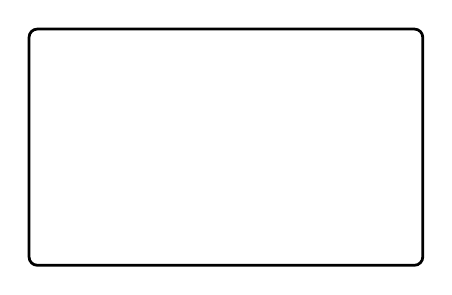
\begin{tikzpicture}\draw[line width=1pt,rounded corners=3pt] (0,0) rectangle (5,3); \end{tikzpicture}\end{center}
\end{puzzle}

\begin{puzzle}{Two keys}
Key X and Key Y both sort the eight bugs into eight groups. Is one of them wrong? \wline[2cm] How would you decide which is better? \wline[4cm]
\end{puzzle}

\begin{puzzle}{Clear or fuzzy?}
Write C for clear or F for fuzzy.\\
(a) Has four legs \wline[1cm] \quad (b) Is bright \wline[1cm] \quad (c) Longer than 5~cm \wline[1cm] \quad (d) Looks happy \wline[1cm]
\end{puzzle}

\begin{puzzle}{Not told}
Why must your friend not be told the answers before using the key? \wline[6cm]
\end{puzzle}

\begin{puzzle}{Your trade}
Trade keys with a friend. How many of ten matched? \wline[1.6cm] Which question was the problem? \wline[4cm]
\end{puzzle}
\clearpage
\thispagestyle{fancy}
\subhead{Trade record}
Record each trade. Write the question that caused disagreement and the change you made.\par\medskip
\renewcommand{\arraystretch}{3.0}
\begin{tabularx}{\linewidth}{|>{\sffamily\small\bfseries}p{1.8cm}|X|X|X|}
\hline
Trade & Agreed (of 10) & Question that caused trouble & My fix \\ \hline
1 & & & \\ \hline
2 & & & \\ \hline
3 & & & \\ \hline
4 & & & \\ \hline
\end{tabularx}

\vspace{8pt}
After the last fix, did a new friend agree on all ten? \wline[3cm]\\[10pt]
What is one thing you learned about writing questions? \wline[6cm]
\clearpage
